\documentclass[11pt,a4paper]{letter}
\usepackage[utf8]{inputenc}
\usepackage[english]{babel}
\usepackage{amsmath}
\usepackage{amsfonts}
\usepackage{amssymb}
\usepackage{tikz}\usetikzlibrary{arrows, calc,decorations.markings,cd}
\usepackage[left=3.5cm,right=3.5cm,top=2.5cm,bottom=4cm]{geometry}

\begin{document}
\pagestyle{empty}
Something goes wrong with these braid matrices. Let me illustrate. If
\begin{center}
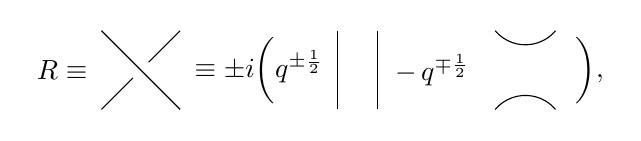
\begin{tikzpicture}
\node (R) at (-1,0) {$R \equiv$};
\draw (-.5,.5) -- (.5,-.5);
\draw (-.5,-.5) -- (-0.1,-0.1);
\draw (0.1, 0.1) -- (.5,.5);
\node (eq) at (1.5,0) {$\equiv \pm i \biggl( q^{\pm \frac{1}{2}}$};
\draw (2.5,.5) -- (2.5,-.5);
\draw (3,.5) -- (3,-.5);
\node (minus) at (3.7,0) {$-\,q^{\mp \frac{1}{2}}$};
\draw (4.5,0.5) arc[start angle=220, end angle=320, radius=0.5];
\draw (4.5,-0.5) arc[start angle=140, end angle=40, radius=0.5];
\node (bl) at (5.7,0) {$\biggr),$};
\end{tikzpicture}
\end{center}
then we can clearly drop the $\pm i$ when calculating $RR^\dagger$, since they will eliminate to 1 in that product. Let $\widetilde{R}\equiv \mathfrak{Im}(R)$. The coefficients in $\widetilde{R}$ are real, so it is self adjoint. This means we can invoke the Binomial theorem to calculate $RR^\dagger$, and we obtain
\begin{center}
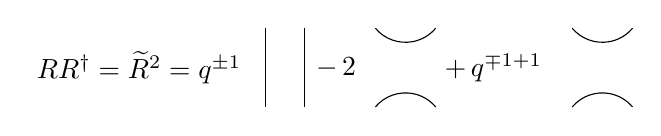
\begin{tikzpicture}
\node (R) at (-2,0) {$RR^\dagger = \widetilde{R}^2 = q^{\pm 1}$};
\draw (-0.4,.5) -- (-.4,-.5);
\draw (.1,.5) -- (.1,-.5);
\node (2nd) at (0.5,0) {$-\,2$};
\draw (1,0.5) arc[start angle=220, end angle=320, radius=0.5];
\draw (1,-0.5) arc[start angle=140, end angle=40, radius=0.5];
\node (3rd) at (2.5,0) {$+\, q^{\mp 1 + 1}$};
\draw (3.5,0.5) arc[start angle=220, end angle=320, radius=0.5];
\draw (3.5,-0.5) arc[start angle=140, end angle=40, radius=0.5];
\end{tikzpicture}
\end{center}
The $+1$ in the last term (in the exponent) comes from eliminating a loop.

For the two possible choices of signs, the coefficients of \,
\tikz[baseline=-1.5mm, scale=0.5]{\draw (3.5,0.5) arc[start angle=220, end angle=320, radius=0.5];
\draw (3.5,-0.5) arc[start angle=140, end angle=40, radius=0.5];}
are given by $-1$ and $-(2-q^2)$, the latter being equal to 0 iff $q = 2\cos{\frac{\pi}{4}}$.

Therefore, $R$ is, in general, not perfect. So either there is a major misunderstanding here, or (this is what I believe) $R$ is somehow defined incorrectly.

\bigskip\noindent
I believe that because I too have verified that a tangle of the form 
\begin{center}
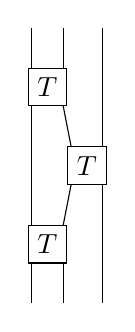
\begin{tikzpicture}
\node[draw] (T1) at (0,1) {$T$};
\node[draw] (T2) at (0.5,0) {$T$};
\node[draw] (T3) at (0,-1) {$T$};
\draw ($(T1.south) + (-0.2,0)$) -- ($(T3.north) + (-0.2,0)$);
\draw ($(T1.south) + (0.2,0)$) -- ($(T2.north) + (-0.2,0)$);
\draw($(T3.north) + (0.2,0)$) -- ($(T2.south) + (-0.2,0)$);
\draw ($(T2.south) + (0.2,0)$) -- ($(T2.south) + (0.2,-1.5)$);
\draw ($(T2.north) + (0.2,0)$) -- ($(T2.north) + (0.2,1.5)$);

\draw ($(T3.south) + (0.2,0)$) -- ($(T3.south |- T2.south) + (0.2,-1.5)$);
\draw ($(T3.south) + (-0.2,0)$) -- ($(T3.south |- T2.south) + (-0.2,-1.5)$);

\draw ($(T1.north) + (0.2,0)$) -- ($(T1.north |- T2.north) + (0.2,1.5)$);
\draw ($(T1.north) + (-0.2,0)$) -- ($(T1.north |- T2.north) + (-0.2,1.5)$);
\end{tikzpicture}
\end{center}
is perfect if $T$ is perfect. 

\begin{flushright}\boxed{
\begin{minipage}{0.8\textwidth}
By the way: Last time I have said that there's no harm in defining \emph{perfectness} by saying: all the `rotated multiplications' are \underline{equal} to $\mathrm{id}_k$, instead of \underline{proportional}. That is not quite true, because: if we partitioned the legs of e.g.\ a 3-tangle into sets of size 2 and 4, then for these bipartitions the product is $q\cdot\mathrm{id}_2$, i.e.\ this notion of \emph{perfectness} would not be downward compatible, in a sense. So we should probably stick with proportionality.

~\\ But I guess we could get sort of a ``generating set'' $S$ for perfect tangles (the generating operation being rotation, if we require that the coefficient of $\mathrm{id}_k$ of $T\in S$ be of modulus 1. Does that make sense to you? After a bit of thinking I suppose that this is not in fact generating all perfect tangles.
\end{minipage}}
\end{flushright}

I do not see how the Reidemeister moves force this tangle to be perfect, though -- I guess I might need to carefully work through section \textbf{2.11} in \emph{Planar Algebras, I}.

While it is not entirely clear to me how the generalization at the end of your notes works, I interpreted it so that I get, for example, the following 4-tangle:
\begin{center}
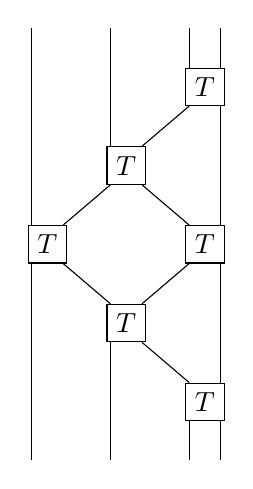
\begin{tikzpicture}
\node[draw] (T1) at (0,0) {$T$};
\node[draw] (T2) at (1,1) {$T$};
\node[draw] (T3) at (1,-1) {$T$};
\node[draw] (T4) at (2,2) {$T$};
\node[draw] (T5) at (2,0) {$T$};
\node[draw] (T6) at (2,-2) {$T$};

\path ($(T1.north) + (-0.2,0)$) edge ($(T1.north |- T1.north) + (-0.2,2.5)$)
	($(T2.north) + (-0.2,0)$) edge ($(T2.north |- T1.north) + (-0.2,2.5)$)
	($(T4.north) + (-0.2,0)$) edge ($(T4.north |- T1.north) + (-0.2,2.5)$)
	($(T4.north) + (0.2,0)$) edge ($(T4.north |- T1.north) + (0.2,2.5)$);

\path ($(T1.south) + (-0.2,0)$) edge ($(T1.south |- T1.south) + (-0.2,-2.5)$)
	($(T3.south) + (-0.2,0)$) edge ($(T3.south |- T1.south) + (-0.2,-2.5)$)
	($(T6.south) + (-0.2,0)$) edge ($(T6.south |- T1.south) + (-0.2,-2.5)$)
	($(T6.south) + (0.2,0)$) edge ($(T6.south |- T1.south) + (0.2,-2.5)$);

\path ($(T1.north) + (0.2,0)$) edge ($(T2.south) + (-0.2, 0)$)
 ($(T2.north) + (0.2,0)$) edge ($(T4.south) + (-0.2, 0)$);
 
 \path ($(T1.south) + (0.2,0)$) edge ($(T3.north) + (-0.2, 0)$)
 ($(T3.south) + (0.2,0)$) edge ($(T6.north) + (-0.2, 0)$);
 
\path ($(T2.south) + (0.2, 0)$) edge ($(T5.north) + (-0.2, 0)$)
	($(T3.north) + (0.2,0)$)  edge ($(T5.south) + (-0.2, 0)$);
	
\path ($(T4.south) + (0.2,0)$) edge ($(T5.north) + (0.2, 0)$)
	($(T6.north) + (0.2,0)$)  edge ($(T5.south) + (0.2, 0)$);
\end{tikzpicture}
\end{center}
And now buckle up: This is perfect (given that both $T$ is perfect and I did not make a mistake). This would be the first example of a perfect 4 tangle! Quite exciting. But I don't understand why this construction works. Did Vaughan make that up on the spot, or has he thought about it before?

I have to prove that this construction yields perfect $k$-tangles for all $k$, but I can check whether this is true for $k=6$, which is apparently a case Vaughan is interested in. In general such a $k$-tangle would consist of $\frac{k(k-1)}{2}$ internal boxes. So on 6 strands there would be 15 boxes, which is tedious but doable.

The nice thing about tangles $M$ of this form, though, is that one only has to check the cases $\mathrm{rot}^l M \cdot \mathrm{rot}^{-l}M^\dagger$ for $0\leq l < k$, since they are highly symmetric. 

\hrulefill

Addendum: I have tried generalizing this to $T$ being a $3$-box, but it was not successful, I tried about 5 different ways, didn't work.

\end{document}